\chapter*{Introduction}
First introduced in 1851, as part of Bernhard Riemann's doctoral
thesis\sidenote{\footnotesize\cite{riemann}}, Riemann surfaces have been central
to the development of mathematics in the 20$^{\mathrm{t h}} $ and 21$
	^{\mathrm{s t}} $ centuries. This publication sparked the rigorous and
methodical study of topology, and was responsible for drawing significant links
between complex analysis and algebraic geometry, an area essentially born of the
thesis. Riemann's discovery of these objects is representative of the
unification of many previously explored branches of theory, and this influence
is evident by the naming of key theorems throughout, for example with Abel's
addition theorem, and the Jacobi inversion theorem.

The first exploration of the concept, by Riemann himself, was concerned with
branches of multivalued complex functions, for example, the square root. Riemann
had the idea (``one of the most illuminating in the history of
mathematics''\sidenote{\footnotesize\cite{stillwell}}) to represent the relation
$ p ( x,y )=0 $ between $ x,y \in \mathbb{C} $ by covering a plane representing
the values of $ x $, by a surface representing the values of $ y $. We will
explore this idea and those related in Section~\ref{sec:affine-curves}.

\begin{figure}[h]
	\centering
	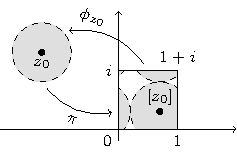
\includegraphics{sqrt-covering/figure}
	\caption{Freely deforming the unit disk such that the points $ y = \pm\sqrt{x}
		$ lie above $ x $.}
\end{figure}

The study of Riemann surfaces has behind it two remarkably distinct trails of
research and theory, paved respectively by complex manifold theory, and
algebraic geometry. We tend to explore the subject through the former
characterisation, but ommission of key results and ideas arising from the latter
would be misguided. As a result, there are chapters and sections of the report
which take more explicit notice of the algebraic geometric development, although
these are somewhat less integral to our main aim; the Riemann--Roch theorem for
compact Riemann surfaces.

\section*{Acknowledgement}
I am indebted to my project supervisor Raphael Zentner for his numerous resource
recommendations, for pushing me and my project in a direction both interesting
and challenging, and for the provision of herbal tea and chocolate.

